\chapter{Evaluation}
\label{cha:evaluation}
\section{Experiment Environment}
\subsection{Compiler}
Minizinc IDE is a compiler which allows users to edit and run their models, which is developed by the University of Melbourne, Monash University, and Data61 Decision Sciences\cite{r6}. It provides some build-in functions as well as optimization methods. In our models, the build-in Minizinc-to-Flatzinc translator and AC3 has been applied. In addition, A wide range of solvers has been tested.
\begin{itemize}
    \item Choco: A JAVA CSP solver, which supports many search strategies (DomWDeg, ABS, IBS, first-fail, etc.) and optimization processes (LNS, fast restart).
    \item Chuffed: A C++ FD solver using lazy clause generation, which contains a nogood logbook to avoid plenty of duplicate calculation.
    \item Coin-bc: A C++ based Mixed Integer Programming (in our case, the MIP model is the same with CSP model) solver, it adopts the branch and cut optimization.
    \item Gurobi: A commerical solver support MIP.
    \item Izplus: Based on iZ-C constraint programming that is developed by NTT DATA SEKISUI SYSTEMS CORPORATION. It combines Randomized restarting, Local search, Variable reordering and NG learning.
    \item Jacop: A JAVA CSP solver.
    \item Or-tool: An open-source solver developed by google, it combines many optimization methods.
    \item PicatSAT: A CSP solver based on picat which is a rule-based language. And it adopts log encoding~\cite{r8}.
    \item Yuck: Based on scala and combines local search with restarting, global constraints, and lexicographic cost functions.
\end{itemize}
\subsection{Software Platform}
\label{sec:softplat}
All the experiments based on the Windows subsystem for Linux 2 (WSL2) which allows the developer run a Linux environment on Windows 10. Table~\ref{tab:Ubuntu} shows the version of the WSL2.
\begin{table*}[htbp]
  \centering

  \caption{The version of Windows subsystem for Linux}
  
  \label{tab:Ubuntu}
  \input table/Ubuntuversion.tex
\end{table*}
In addition, there are nine solvers has been applied in our experiment, Table~\ref{tab:solvers} indicates the version of each solver.
\begin{table}[htbp]
  \centering

  \caption{The solvers and corresponding versions}
  
  \label{tab:solvers}
  	\begin{subtable}[b]{\textwidth}
  	\centering
  \input table/solver1.tex
    \end{subtable}\\
    	\begin{subtable}[b]{\textwidth}
  	\centering
  \input table/solver2.tex
  \end{subtable}\\
  \begin{subtable}[b]{\textwidth}
  \centering
  \input table/solver3.tex
  \end{subtable}
\end{table}
\subsection{Hardware Platform}
\label{sec:hardplat}

\begin{table*}[htbp]
  \centering

  \caption{Processors used in our evaluation}
  
  \label{tab:machines}
  \input table/machines.tex
\end{table*}


\section{Result}
\label{sec:Result}
In this section, both the results of IQ Twist experiments and the results of Zig Zag Puzzler will be discussed. The discussions will mainly include two parts, the coverage and the average time of each solver.
\subsection{IQ Twist Result}
\label{sec:IQtwistresult}
Generally, all the cases in the IQ Twist booklet has been tested by the nine solvers. There is a total of 120 cases for each solver, which consists of five difficulties 'start', 'junior', 'expert', 'master' and 'wizard'. Each difficulty contains 24 cases. For each case, the time limit is 30 minutes. If the solver can get the result in 30 minutes, the time will be logged, otherwise, we treat it as a unsolved case.
\\Firstly, for each solver, we can calculate the coverage rates by the Equation
\begin{equation}
   C= N1/N2\times 100\% ,
\end{equation}
where $C$ means the coverage rates, $N1$ means the number of solved cases and $N2$ means the number of total cases.
\begin{figure}[htbp]
    \centering
    \begin{subfigure}[b]{0.48\textwidth}
    \centering
    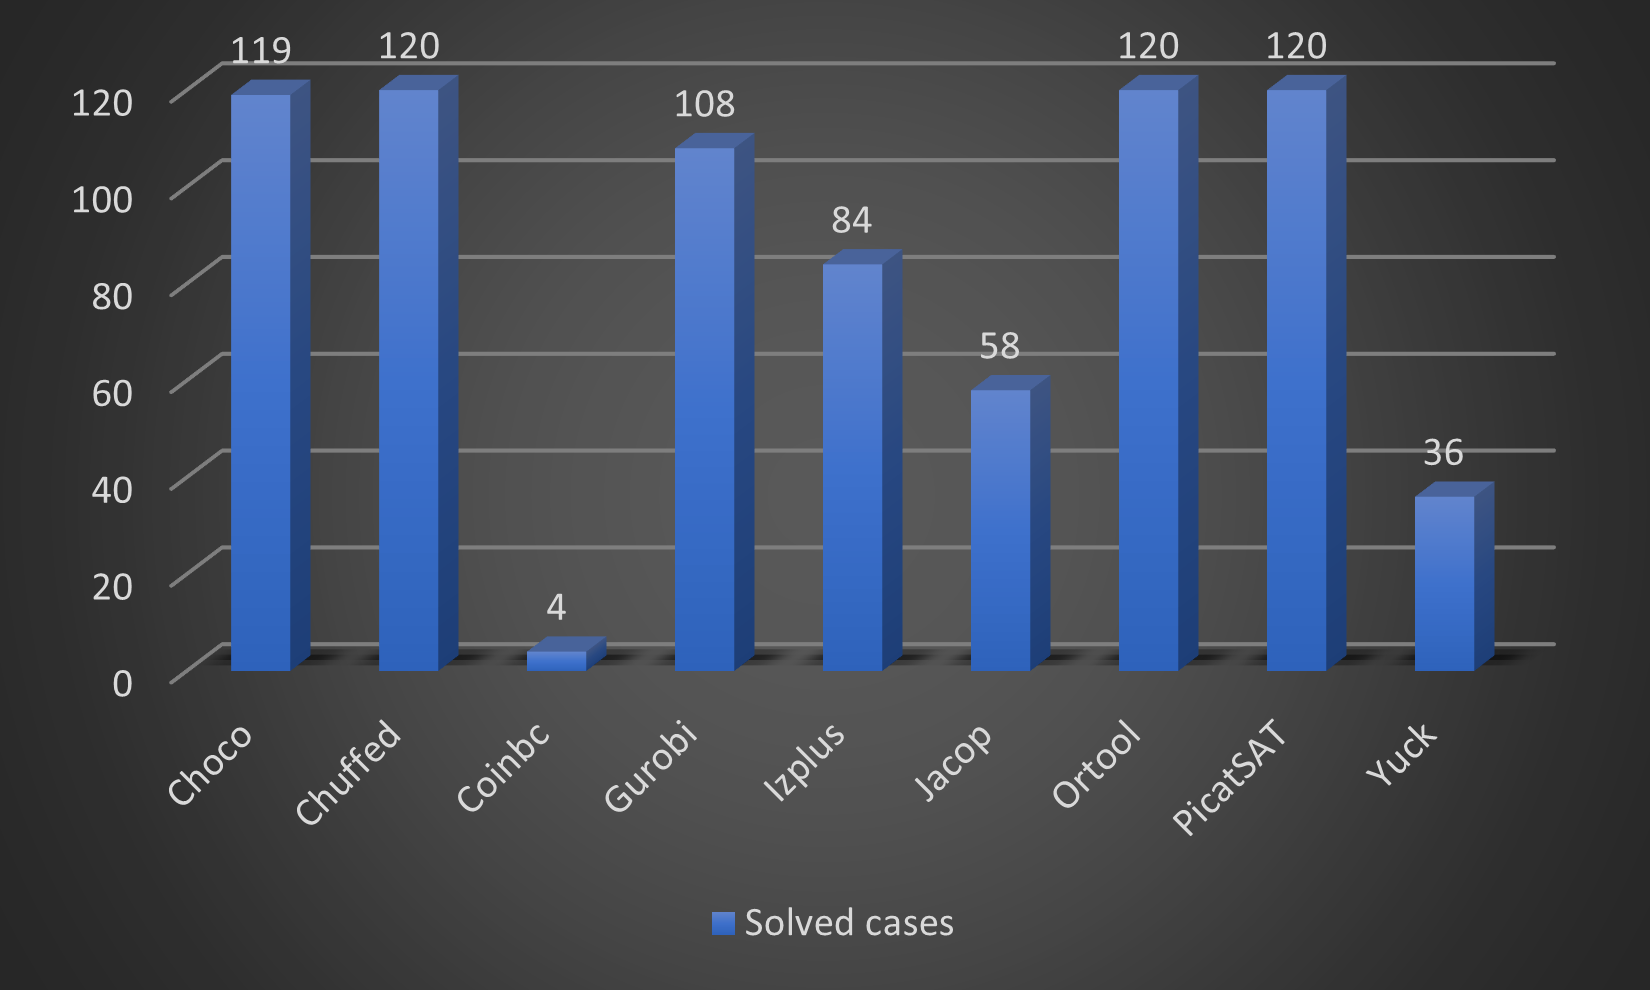
\includegraphics[width=\textwidth]{figs/solvedcases.png}
    \caption{The number of solved cases for each solver}
    \label{eva1}
    \end{subfigure}
     \begin{subfigure}[b]{0.48\textwidth}
     \centering
    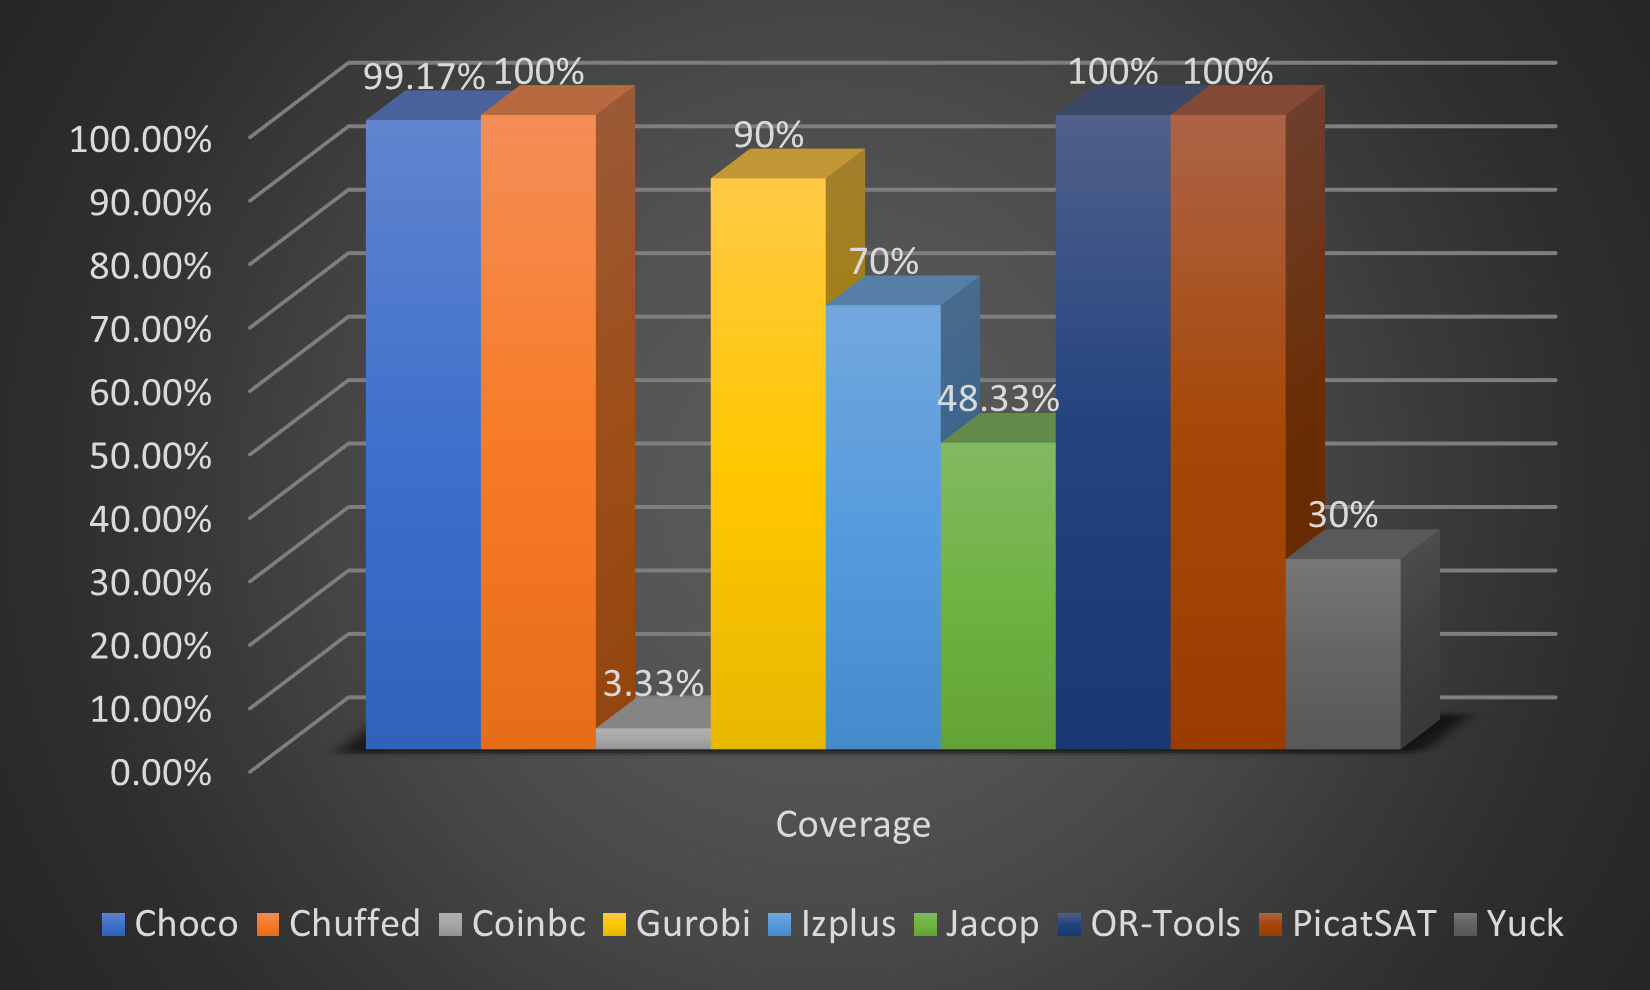
\includegraphics[width=\textwidth]{figs/coverage.png}
    \caption{Overall coverage rates of each solver}
    \label{eva2}
    \end{subfigure}
     \begin{subfigure}[b]{0.48\textwidth}
    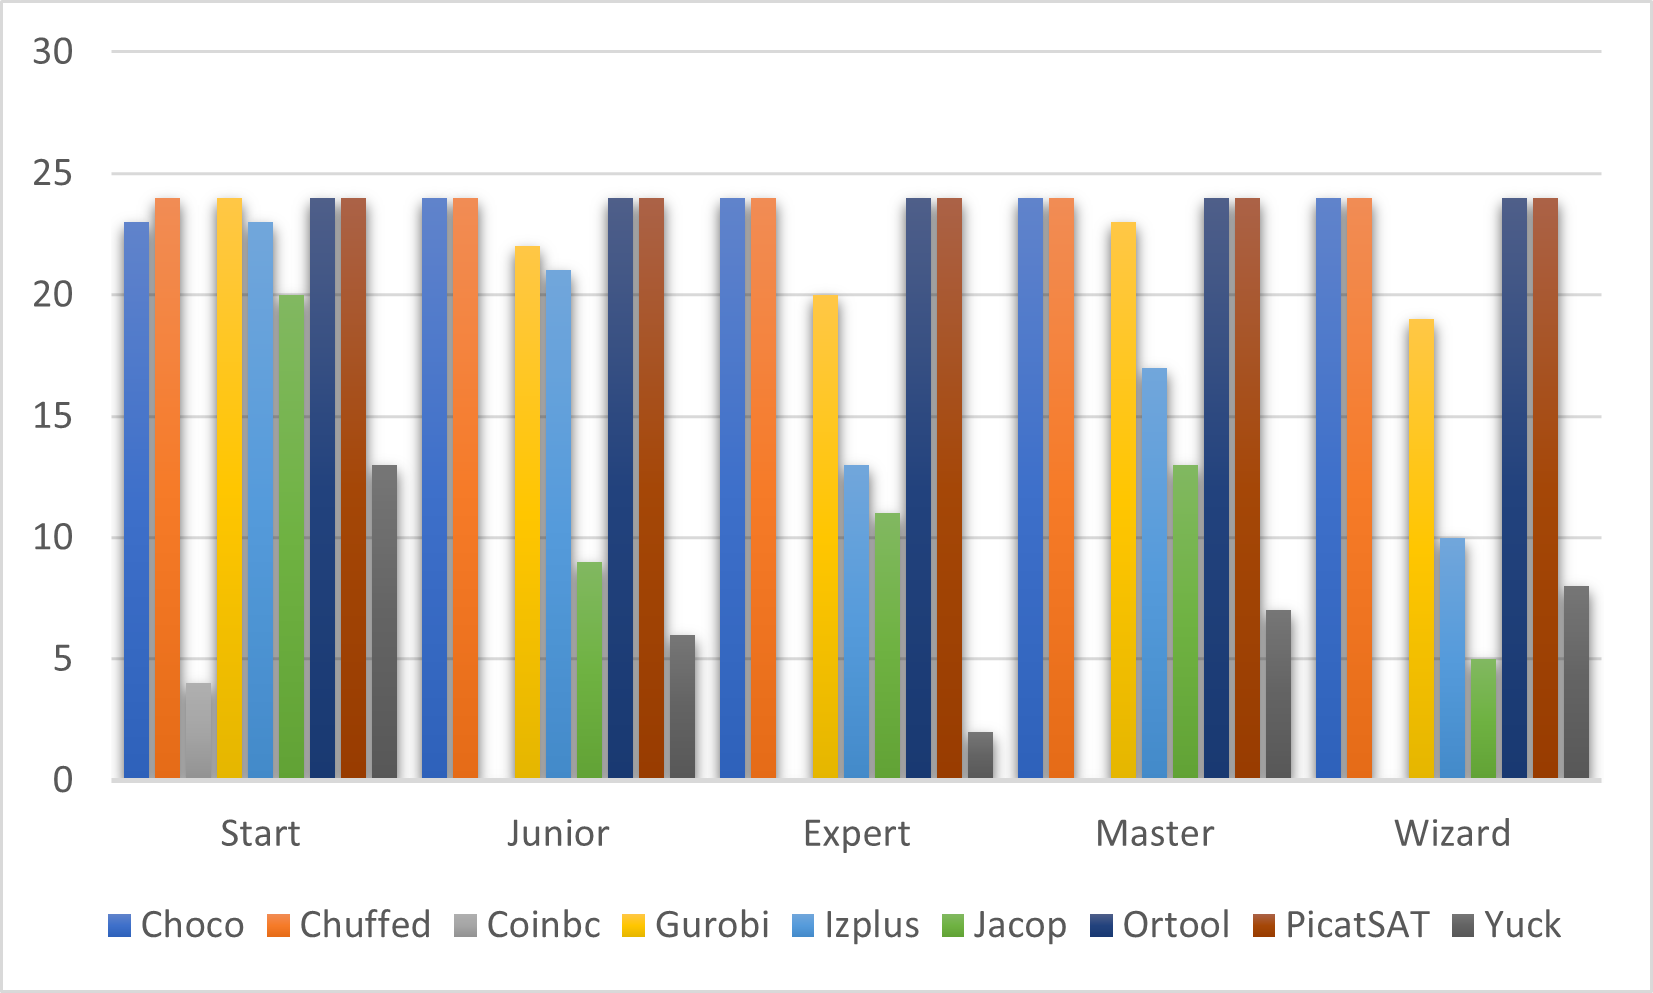
\includegraphics[width=\textwidth]{figs/separated number.png}
    \caption{The number of solved cases of each difficulty for each solver}
    \label{eva3}
    \end{subfigure}
    \begin{subfigure}[b]{0.48\textwidth}
    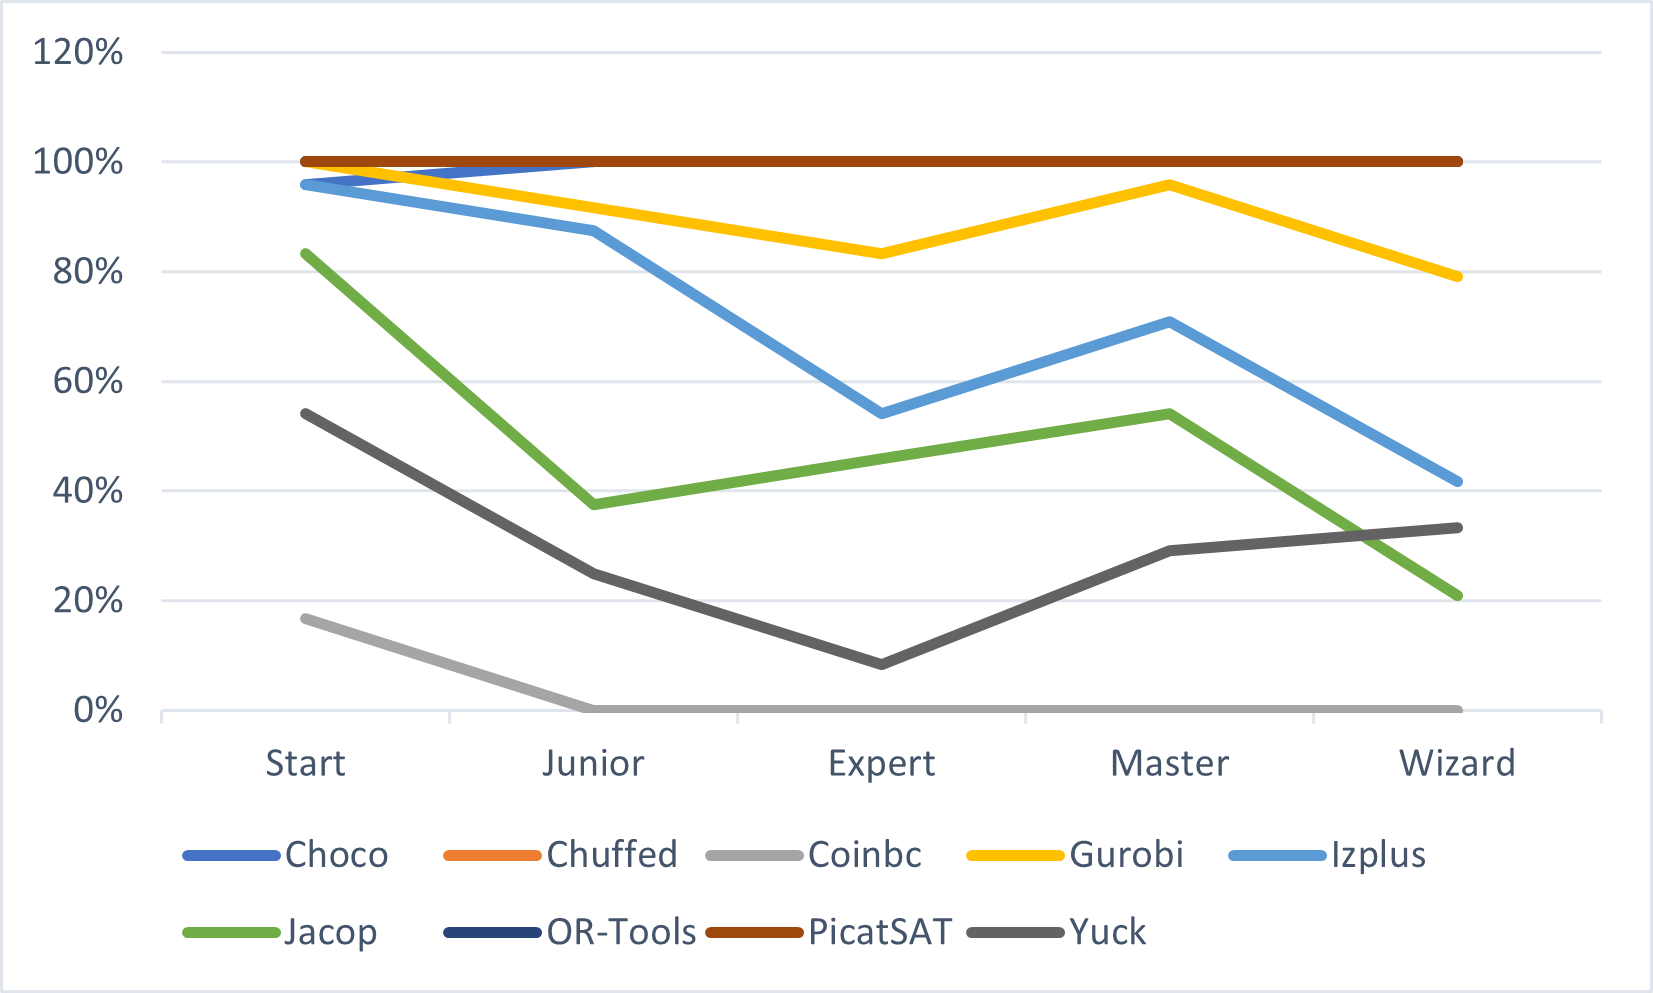
\includegraphics[width=\textwidth]{figs/separated coverage.png}
    \caption{The coverage rates of each difficulty for each solver}
    \label{eva4}
    \end{subfigure}
    \caption{Coverage rates and the number of solved cases in IQ Twist}
    \label{fig:comparisonIQtwist}
\end{figure}
Figure~\ref{eva1} shows the overall solved cases for each solver. Based on the data in Figure~\ref{eva1}, Figure~\ref{eva2} shows the overall coverage rates for different solvers, which indicates that there are only 3 solvers' overall coverage rates are 100 percentage. In addition, Figure~\ref{eva3} separately shows the solved cases for different difficulties for each solver. Accordingly, Figure~\ref{eva4} reveals the change of coverage rates as the increasing of difficulty. It seems like that the other solvers are not stable except the 3 solvers which always keep 100 percentages. Therefore, compared with other solvers, Picat, Ortool and Chuffed take advantages in coverage rates.
\\In addition, based on the solved cases, we calculate the average execution time for each solver by
\begin{equation}
\overline{t}=\frac{\sum\limits_{i=1}^n t_{i}}{n},
\end{equation}
where $\overline{t}$ is the average execution time, $\sum\limits_{i=1}^n t_{i}$ is the sum of each execution time for solved cases and $n$ is the number of solved cases.
\begin{figure}[htbp]
\centering
\begin{subfigure}{0.48\textwidth}
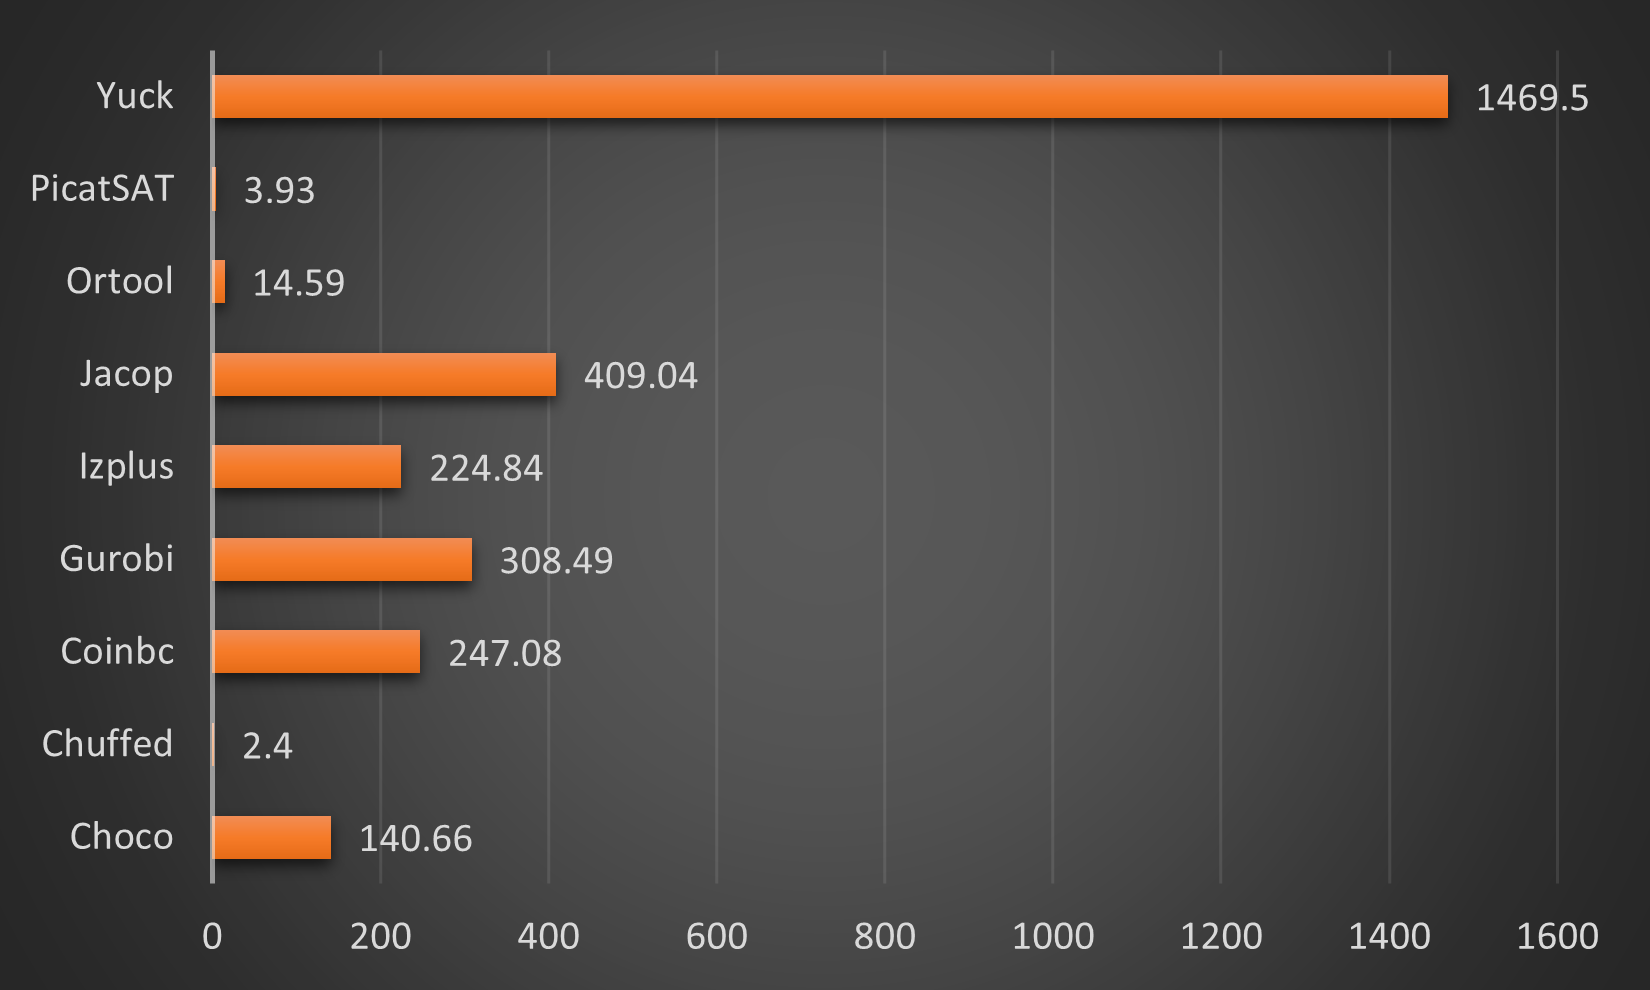
\includegraphics[width=\textwidth]{figs/averagetime.png}
\caption{The overall average execution time for solved cases}
\label{fig:averagetime1}
\end{subfigure}
\begin{subfigure}{0.48\textwidth}
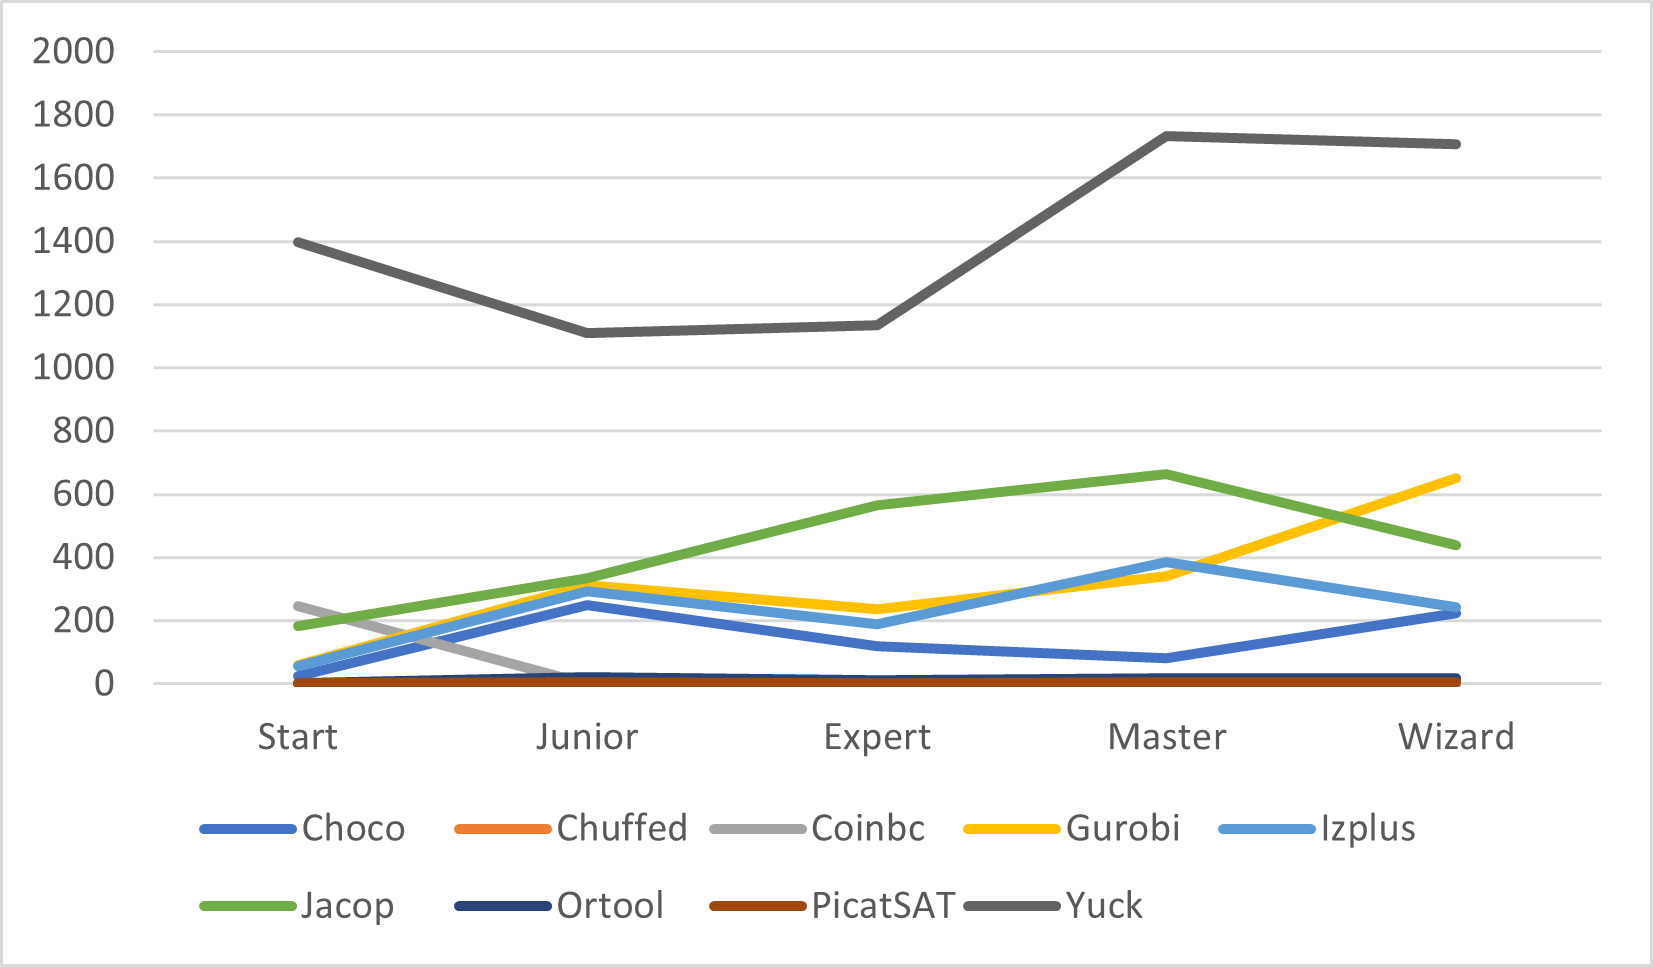
\includegraphics[width=\textwidth]{figs/separated time.png}
\caption{The separated average execution time for solved cases}
\label{fig:averagetime2}
\end{subfigure}
\caption{The average execution time for solved cases}
\label{fig:averagetime}
\end{figure}
Figure~\ref{fig:averagetime} shows the average execution time for each solver. Again, Chuffed, PicatSAT and Ortool takes huge advantages compared with other solvers. In addition, the overall execution times of Chuffed and PicatSAT are close, and they are better than the overall execution time of Ortool. 
\begin{figure}[htbp]
\centering
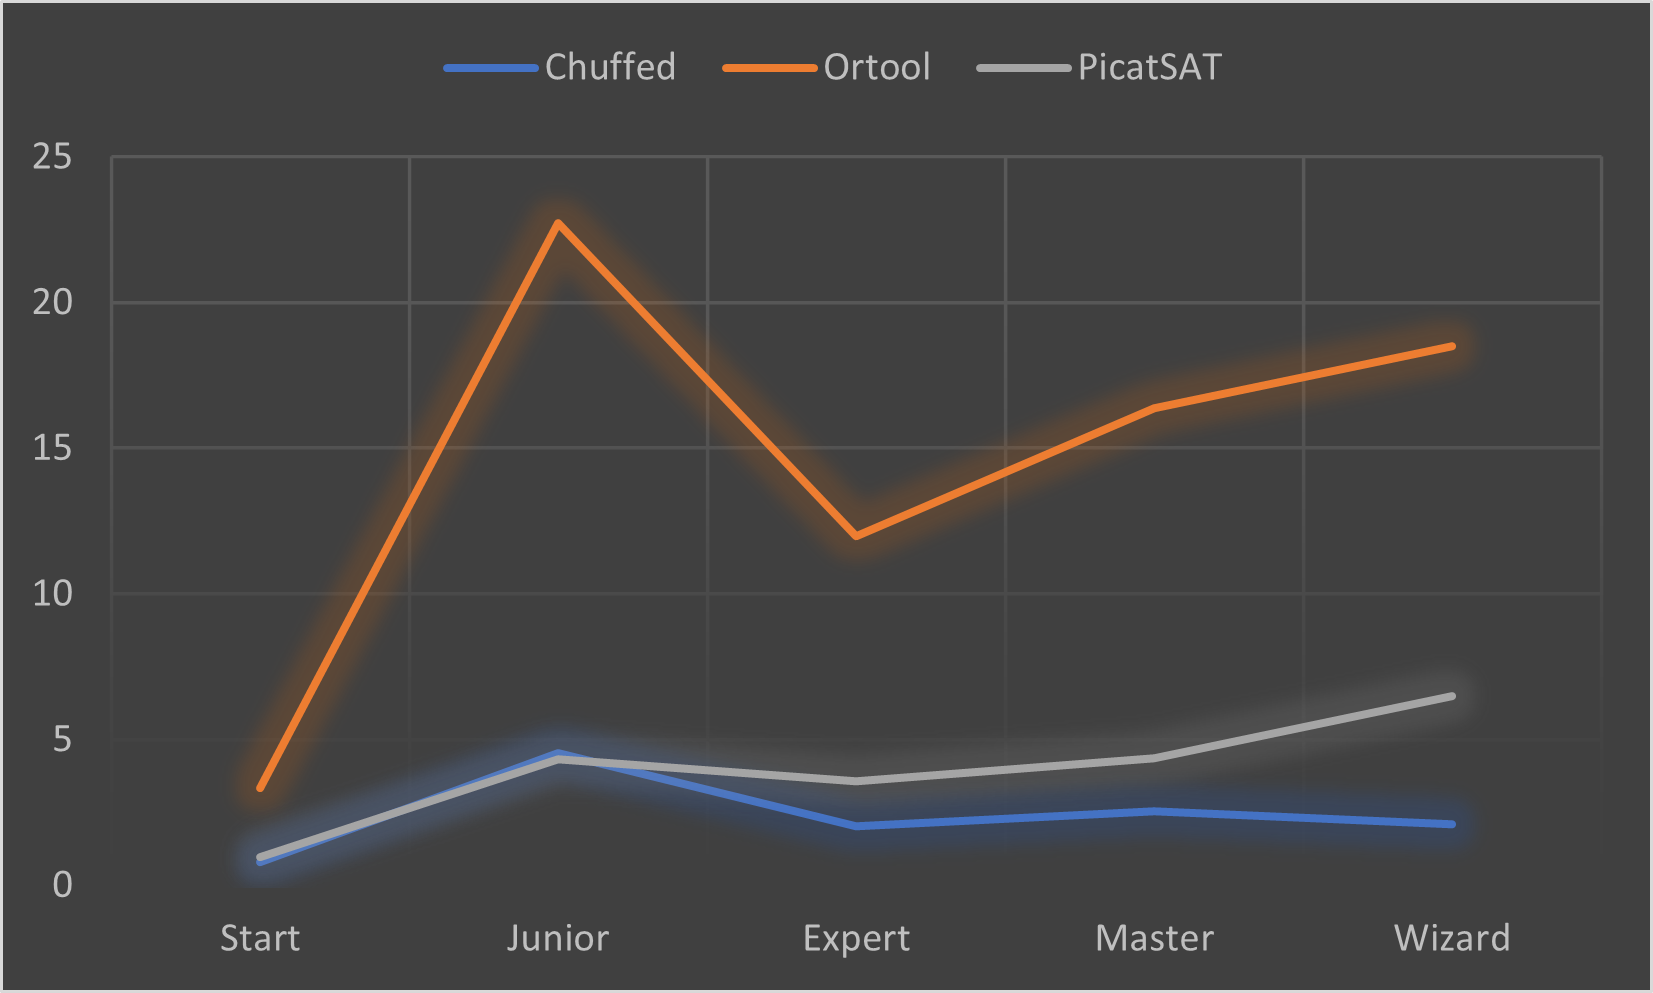
\includegraphics[width=0.6\textwidth]{figs/Three comparison.png}
\caption{The separated execution time comparisons between Chuffed, Picat and Ortool}
\label{fig:3comparison}
\end{figure}
Furthermore, Figure~\ref{fig:3comparison} indicates that the chuffed spends less time than PicatSAT except in the "junior" difficulty.
\\Overall, although Chuffed, PicatSAT and Ortool can get the result for each case in 30 minutes, the Chuffed possesses the best performance in IQ Twist.
\subsection{Zig Zag Puzzler Result}
\label{sec:Zig Zag Puzzlerresult}
Similarly, all the cases in the Zig Zag Puzzler booklet has been tested by the nine solvers. There is a total of 80 cases for each solver, 40 of them belong to playing mode1, and the other 40 belong to playing mode2. For each playing mode, there are 5 difficulties 'start', 'junior', 'expert', 'master', 'wizard'. Each difficulty contains 8 cases. For each case, the time limit is 30 minutes. If the solver can get the result in 30 minutes, the time will be logged, otherwise, we treat it as a unsolved case.